\documentclass[onecolumn, referee]{svjour3}                     % onecolumn (standard format)
\smartqed  % flush right qed marks, e.g. at end of proof
%\documentclass[12pt]{article}
%\documentclass[smallextended]{svjour3}     % onecolumn (second format)
%\documentclass[twocolumn]{svjour3}         % twocolumn
%
%

\usepackage{epsf,amsmath,amsfonts}
\usepackage{graphicx}
%\usepackage{epstopdf}
\usepackage{caption}
\usepackage{amssymb}
\usepackage{bm}
\usepackage{psfrag}
\usepackage{mathptmx}      % use Times fonts if available on your TeX system

\newcommand{\snorm}[1]{{ \|| #1 |\|}}
\newcommand{\double}{\baselineskip 1.5 \baselineskip}
\newtheorem{defn}{Definition}
\newtheorem{thm}{Theorem}
\newtheorem{alg}{Algorithm}

%
%
% insert here the call for the packages your document requires
%\usepackage{latexsym}
% etc.
%
% please place your own definitions here and don't use \def but
% \newcommand{}{}
%
% Insert the name of "your journal" with
%\journalname{Ocean Dynamics}
%
\begin{document}

\title{Vector reconstruction using Radial Basis Function: A working document}

\author{Xylar Asay-Davis \and Todd Ringler}

\authorrunning{Ringler et al.} % if too long for running head

\institute{{\bf Xylar Asay-Davis} \at
              T-3 Fluid Dynamics Group / Center for Nonlinear Studies \\
              Theoretical Division \\
              Los Alamos National Laboratory \\
              Los Alamos, NM 87545
              Tel.: +505-606-0025\\
              \email{xylar@lanl.gov} 
           \and
            {\bf Todd Ringler} \at
              T-3 Fluid Dynamics Group \\
              Theoretical Division \\
              Los Alamos National Laboratory \\
              Los Alamos, NM 87545
              Tel.: +505-667-7744\\
              \email{ringler@lanl.gov}           %  \\
}

\date{Received: date / Accepted: date}
% The correct dates will be entered by the editor

\maketitle

\abstract
When implementing traditional C-grid finite-volume methods, we retain only one component of the full velocity field at each momentum point.  For visualization purposes, in order to compute tracer tendancies, and in order to implement immersed boundary methods it is necessary to have a method for reconstructing the vector field at arbitrary points within each cell.  Here, we outline a method for performing this reconstruction using Radial Basis Functions (RBFs).

%\pagebreak

\section{Requirements}

Given a Voronoi diagram in $\mathbb{R}^2$ spanning domain $\Omega$, we position our momentum points at the midpoint of the line segment connecting the generators, $\bm{g}_k \subset \mathbb{R}^2$.  At each of these momentum points $\bm{x}_i$, where $i$ is the index of the edge, we only retain the component of the velocity in the direction $\bm{\hat{n}}_i$ normal to the cell edge. See Figure \ref{Cgrid}.  We define $u_i$ to be the amplitude of the velocity field in the $\bm{\hat{n}}_i$ direction.  We require a reconstruction $\bm{u}_j(\bm{x})$ at an arbitrary position within the tangent plane of the $j^{\rm th}$ cell.  At least for the time being, the velocities $u_i$ should be members $i \in {\rm edgesOnCell}(j)$, the normal velocities on the edges of the $j^{\rm th}$ cell. (We abbreviate ${\rm edgesOnCell}(j)$ as EOC$(j)$ in the remainder of the text.)

\begin{figure}[ht!]
   \centerline{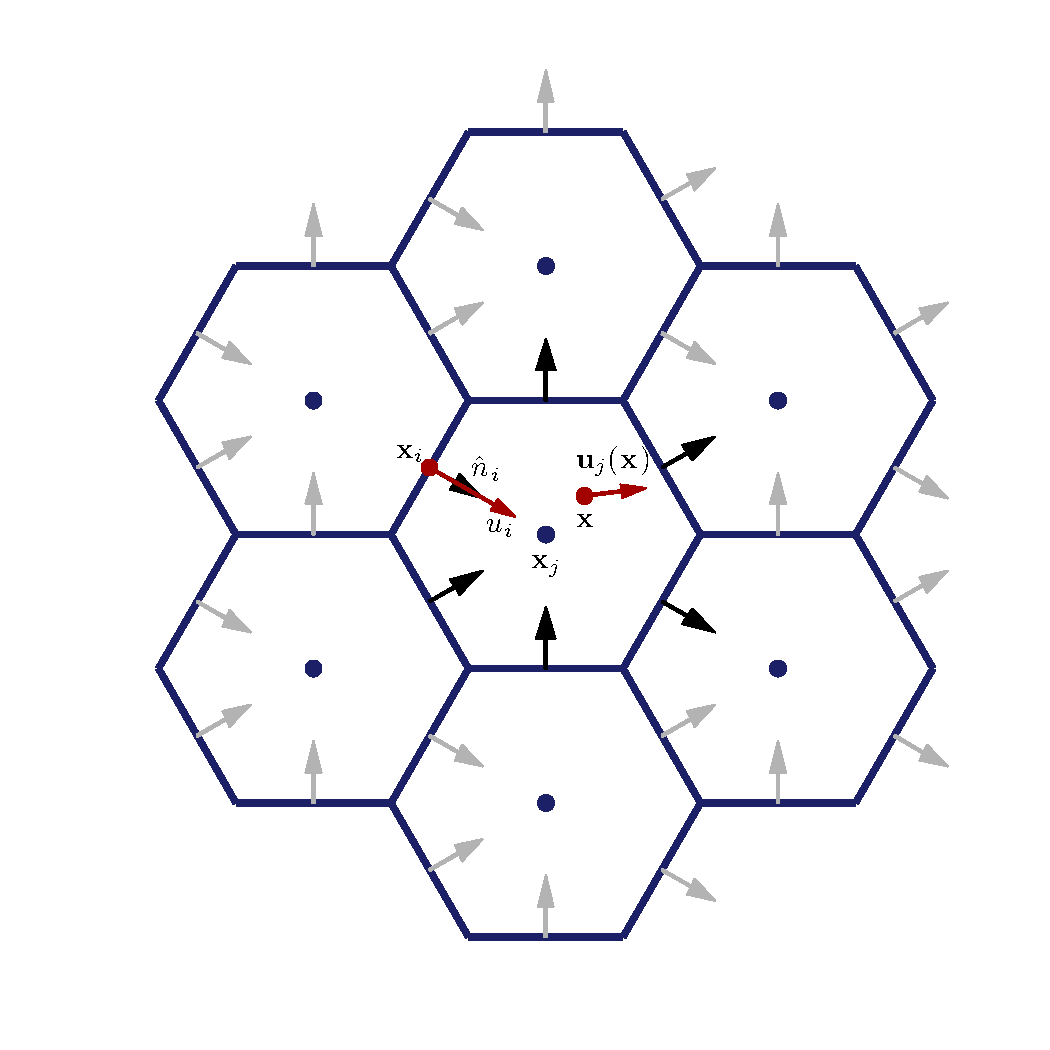
\includegraphics[width=12.0cm]{./figures/cgrid2.pdf}}
   \caption{A schematic of the finite-volume system. The normal component of velocity, $u_i$ is defined at each cell edge. The problem: How do we reconstruct the full velocity $\bm{u}(\bm{x})$ at an arbitrary point in the cell $\bm{x}$ based on the surrounding $u_i$ data?  Of particular interest are the reconstructed velocities at the cell centers $\bm{x}_j$}
   \label{Cgrid}
\end{figure} 

\section{Design}

We base our vector reconstruction on the work of \cite{Ba}.  Given velocity components normal to to the cell edges
\begin{equation}\label{given_data}
u_i = \bm{u}(\bm{x}_i) \cdot  \bm{\hat{n}}_i \quad  i \in {\rm EOC}(j)
\end{equation}
where $N$ is the number of edges on the $j^{\rm th}$ cell, we would like to reconstruct an interpolating velocity within the cell
\begin{equation}\label{problem}
\bm{u}_j(\bm{x}) = \sum_{i \in {\rm EOC}(j)} \bm{c}_i \phi_i(\bm{x}) + \sum_{l=1}^M \bm{d}_l p_l(\bm{x}),
\end{equation}
where $\bm{c}_i$ and $\bm{d}_l$ are vector value coefficients determined by the method described below, $\phi_i(\bm{x})$ is the radial basis function (RBF) associated with the $i^{\rm th}$ edge evaluated at the reconstruction point $\bm{x}$, $p_l(\bm{x})$ are low order polynomials, and $M$ is the (small) number of these polynomials included in the reconstruction.

The form of the RBFs is
\begin{equation}\label{problem}
  \phi_i(\bm{x}) \equiv \phi(\left|\bm{x}-\bm{x}_i\right|),
\end{equation}
where $\phi(r)$ can take any of several forms incuding Gaussian, $\phi(r) = e^{-r^2/(2 \alpha^2)}$ or the inverse mulitquadratic, $\phi(r) = 1/\sqrt{1 + r^2/\alpha^2}$, and where $\alpha$ is a length scale which is on the order of the horizontal cell size.  We have typically used the inverse multiquadratic form with $\alpha$ equal to the average distance between the cell center and the cell edges.

The reconstruction has $2 N + 2 M$ degrees of freedom.  We constrain $N$ of these degrees of freedom by requiring that the reconstruction $\bm{u}_j(\bm{x})$ exactly reproduce the value $u_i$ at the $i^{\rm th}$ edge.  That is,
\begin{align}\label{reproduce_data}
  u_i = & \bm{u}_j(\bm{x}_i) \cdot  \bm{\hat{n}}_i, \nonumber \\
    = & \sum_{i' \in {\rm EOC}(j)} \bm{c}_{i'}\cdot  \bm{\hat{n}}_i \phi_{i'}(\bm{x}_i) + \sum_{l=1}^M \bm{d}_l \cdot  \bm{\hat{n}}_i p_l(\bm{x}_i).
\end{align}
A further $N$ degrees of freedom can be removed by defining $\bm{c}_{i} \equiv c_i \bm{\hat{n}}_i$, so that the $i^{\rm th}$ edge contributes only to the reconstruction of the velocity component normal to that edge.

In general, there will be redundancy between the RBFs and the polynomial basis functions used in the reconstruction.  We constrain the remainig $2 M$ degrees of freedom by requiring that, for each polynomial $p_l(\bm{x})$, the projection of the RBF terms (those involving $c_i$) onto the polynomial evaluated at the corresponding edge point is zero:
\begin{equation}\label{constraint}
  \sum_{i \in {\rm EOC}(j)} c_i \bm{\hat{n}}_i p_l(\bm{x}_i) = 0 \quad  \forall \quad 1 \leqslant l \leqslant M.
\end{equation}
These constraints can be thought of as insuring that tehre is no contribution from each polynomial $p_l(\bm{x})$ to the {\it total} RBF reconstruction $\sum_{i \in {\rm EOC}(j)} c_i \bm{\hat{n}}_i \phi_i(\bm{x})$.

Together, Eqns.~(\ref{reproduce_data}) and (\ref{constraint}) can be expressed as a linear system of the form
\begin{align}\label{linear_system}
  \bm{A} \bm{c} + \bm{P} \bm{d}  = \bm{u}, \\
  \bm{P}^T \bm{c} = \bm{0},
\end{align}
where $A_{i,j} = \bm{\hat{n}}_i \cdot \bm{\hat{n}}_j \phi_{j}(\bm{x}_i)$ and $P_{i,2 l+m} = \hat{n}_{i,m}  p_l(\bm{x}_i)$, $m = 1,2$ corresponding to two arbitrarily chosen unit vectors in the tangent plane of the cell.

So far, we have only tested constant and linear polynomials in our reconstruction.  There is a complication with linear
polynomials: When reconstruction is performed using only the face normals of a given cell (so not including faces from adjacent 
cells), the linear system has a null space of the form
\begin{equation}\label{null_space}
  p_{\rm null}(\bm{x}) = (x \bm{\hat{y}} - y \bm{\hat{x}}),
\end{equation}
which represent local solid body rotation.  The fact that this null space exists should not be a surprise, since we can only represent divergent and not rotating linear flows by using vectors normal to the cell faces.  The null space is derived as follows:
First, assume that all normals point away from the cell center, which is taken to be the origin of the local horizontal reconstruction.  This restriction on the normal vectors can be expressed as
\begin{equation} \label{outward_normal}
  \frac{x_i}{n_{i,x}} = \frac{y_i}{n_{i,y}}, 
\end{equation}
where $x_i$ and $y_i$ are the positions of the $i^{th}$ face of the cell in the local horizontal coordinate system, and $n_{i,x}$ and $n_{i,y}$ are the components of $\bm{\hat{n}}$ in this coordinate system.  If Eq. (\ref{null_space}) is a null space of the matrix
\begin{equation}
  \bm{M} \equiv \left[
  \begin{array}{cc}
     \bm{A} & \bm{P} \\
     \bm{P^T} & \bm{0} 
  \end{array}
  \right],
\end{equation}
then 
\begin{align}
  n_{i,2} p_1(\bm{x_i}) - n_{i,1} p_2(\bm{x_i}) & = 0, \\
  n_{i,y} x_i - n_{i,x} y_i & = 0,
\end{align}
for all $i$,  which is easily rearranged to take the form of Eq. (\ref{outward_normal}).
Similar null spaces may exist for higher order polynomials that have not yet been considered in detail.



\begin{thebibliography}{} 



\bibitem{Ba} {\sc Baudisch, J., L. Bonaventura, A. Iske, and E. Miglio},
	 Matrix-valued radial basis functions for local vector field reconstruction in computational fluid dynamic models, 
	 (2006).
	 
\bibitem{BR} {\sc Bonaventura, L., and T. Ringler},
        Analysis of Discrete Shallow-Water Models on Geodesic Delaunay Grids with C-Type Staggering,
        {\em Mon. Wea. Rev.}, {\bf 133}, pp. 2351?2373, (2005).

\bibitem{Bxx} {\sc Bonaventua, L., }
		Finite Volume Solvers for the Shallow Water Equations Using Matrix Radial Basis Function Reconstruction,
		{\em Numerical Mathematics and Advanced Applications}, pp. 207-214 (2006)

\end{thebibliography}


%\begin{figure}[t]
  % \center{\includegraphics[width=8cm]{./figures/Bamber5km.pdf}}
  % \vspace{1cm}
  % \center{\includegraphics[height=8cm]{./figures/gloutline.pdf}}
  % \caption{\it Top: Distribution of Greenland ice thickness (meters) from \cite{Ba}; Bottom: A piece-wise linear representation
  % of the ice boundary obtained from the ice thickness distribution map.}
  % \label{Bamber}
%\end{figure}




\end{document}
